\section{Derivadas y derivabilidad}


\subsection{Introducción y repaso}
\begin{defn}[Pendiente de una recta]
Sea la recta $y=mx+n$.

Se define \textbf{pendiente de la recta}, $m=\frac{\Delta y}{\Delta x}$
\end{defn}

\begin{defn}[Derivada\IS en un punto]
Se define $f'(a)$ como la derivada de $f(x)$ en el punto $x=a$.

\[f'(a) = \lim_{x\to a}\frac{f(x)-f(a)}{x-a} \overset{(1)}{=} \lim_{h\to 0}\frac{f(a+h)-f(a)}{h}\]

$(1): h=x-a \dimplies x=a+h$

\end{defn}


\begin{example}
Dada $f(x) = |x|$, calcula $f'(0)$.

\[
f(x) = \begin{cases}x&\text{ si } x>0 \\ -x & \text{ si }x\leq 0\end{cases}
\]

Calculamos:

\[
\lim_{x\to 0}\frac{f(x)-f(0)}{x-0} = \begin{cases}
\displaystyle\lim_{x\to 0^+} \frac{f(x)}{x} = \displaystyle\lim_{x\to 0^+} \frac{x}{x} = 1\\\\
\displaystyle\lim_{x\to 0^-} \frac{f(x)}{x} = \displaystyle\lim_{x\to 0^-} \frac{-x}{x} = -1
\end{cases}
\]

\label{derivEjemplo}

Los límites laterales no coinciden, por lo tanto, $\nexists \displaystyle\lim_{x\to 0}\frac{f(x)-f(a)}{x-a} \dimplies \nexists f'(a)$
\end{example}


\subsubsection{Interpretación geométrica de la derivada}

Ver \fref{fig::funinterpretacionderivadapunto}.

\begin{figure}[hbt]
\centering
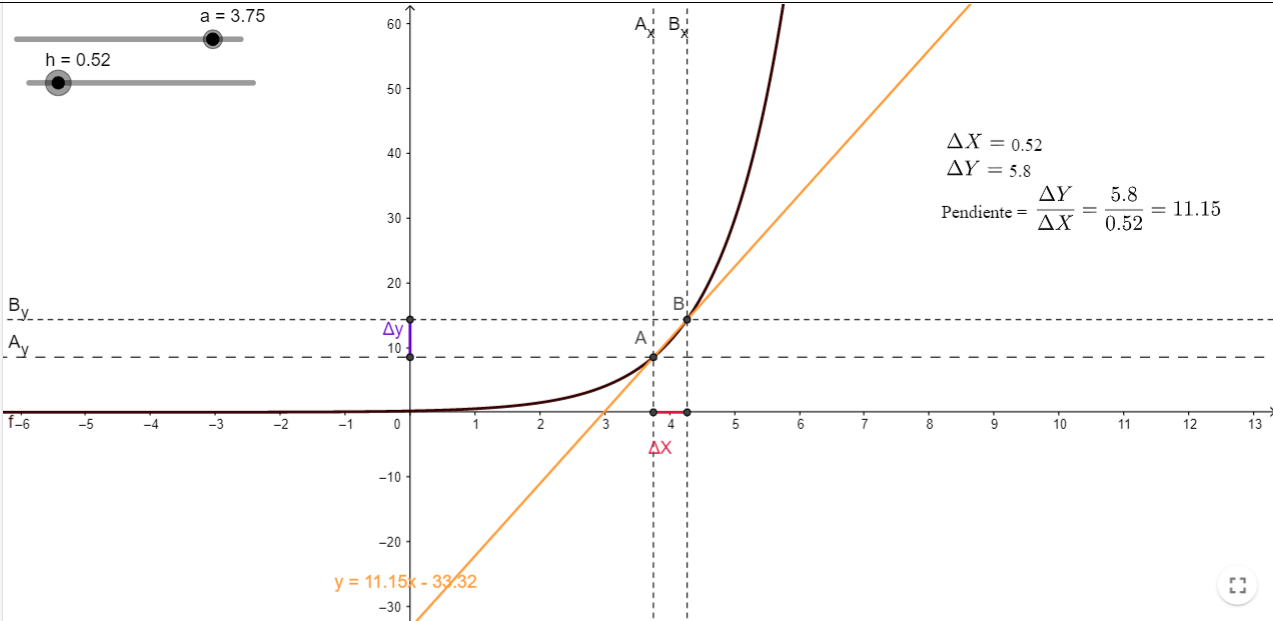
\includegraphics[scale=0.5]{img/DerivadaInterGeometrica}
\label{fig::funinterpretacionderivadapunto}
\caption{Interpretación geométrica de la derivada} Cuando $h\to0$, el punto $B$ se acercará cada vez más al punto $A$, dando lugar a la recta tangente. 
%
Para una mejor comprensión consultar la versión de Geogebra: https://www.geogebra.org/m/jwtw6mdt\#material/f52nQ7T5


\end{figure} 


\subsubsection{Función derivada}

\begin{defn}[Función derivada]
Dada $\appl{f}{D(f)\subset\real}{\real}$. Sea $Dv(f)$ el dominio de derivabilidad de $f$.

La función derivada denotada por $\appl{f'(x)}{Dv(f)\subset\real}{\real}$ hace corresponder a cada $a\in Dv(F)$ el valor $f'(a)$.
\end{defn}

% \begin{table}[hbp]
% \centering
% \begin{tabular}{|c|c|}\hline
% Función & Derivada\\
% \hline
% a&b\\\hline
% \end{tabular}
% \caption{Tabla de derivadas}
% \label{tbl::Derivadas}
% \end{table}



\paragraph{Tabla de derivadas: } Aquí vendría la tabla de derivadas que te dieron el curso pasado. 
%
Si necesitas refrescar cómo se hace una derivada, puedes consultar los vídeos de unicoos sobre las derivadas y la regla de la cadena: \href{https://www.youtube.com/watch?v=m_APcwjkup8}{https://www.youtube.com/watch?v=m\_APcwjkup8}, y \href{https://www.youtube.com/watch?v=Zh0vhnv8Row}{https://www.youtube.com/watch?v=Zh0vhnv8Row}.

\begin{problem}
Hay un PDF en la carpeta con 20 derivadas explicadas.
\solution
\end{problem}

\begin{problem}

\begin{itemize}
	\item 51.58 (2 trigonométricas inversas)
	\item 59.113 (8 variadas. Solo la h tiene una trigonométrica inversa.)
	\item 57.79-81 (Ejercicios resueltos)
\end{itemize}

\solution
\end{problem}
